\documentclass{article}

\usepackage[utf8]{inputenc}
\usepackage[greek, british]{babel}
\usepackage{alphabeta}
\usepackage{libertine}
\usepackage{csquotes}
\usepackage[backend=biber, sorting=none]{biblatex}
\usepackage{hyperref}
\usepackage{graphicx}
\usepackage{float}
\graphicspath{ {./images/} }

\pagenumbering{arabic}

\addbibresource{refs.bib}

\newcommand{\code}{\texttt}

\title{Εργασία Μηχανικής Μάθησης 2022}
\author{Tsirmpas Dimitris}

\begin{document}
	
\maketitle

\section{Λογιστική Παλινδρόμηση}

\subsection{Ερώτημα Δ}
Ο ταξινομητής μας έχει υλοποιηθεί στο αρχείο \code{LogisticRegClassifier.py}. Η πλήρης τεκμηρίωση του μοντέλου, των μεθόδων του και των υπερπαραμέτρων βρίσκεται εκεί με τη μορφή docstrings. Η κανονικοποίηση $L_{2}$ έχει ήδη υλοποιηθεί σε αυτό το αρχείο, αλλά για τους σκοπούς αυτής της ερώτησης θα θέσουμε την υπερπαράμετρο \code{$\lambda$} ως 0, παρακάμπτοντας την.\par

Ο κώδικας για την εκτέλεση του μοντέλου βρίσκεται στο αρχείο \code{run\_logistic.py}. Θα τρέξουμε το μοντέλο με υπερπαραμέτρους \code{iter = 500} και \code{alpha = 0.2}. Το αποτέλεσμα είναι η ακρίβεια εκπαίδευσης να είναι ίση με $0.982$ και η ακρίβεια ελέγχου ίση με $0.981$. Τα πλήρη αποτελέσματα της εκπαίδευσης και του ελέγχου παρουσιάζονται στην Εικόνα \ref{logistic_train_test}.

\begin{figure}
	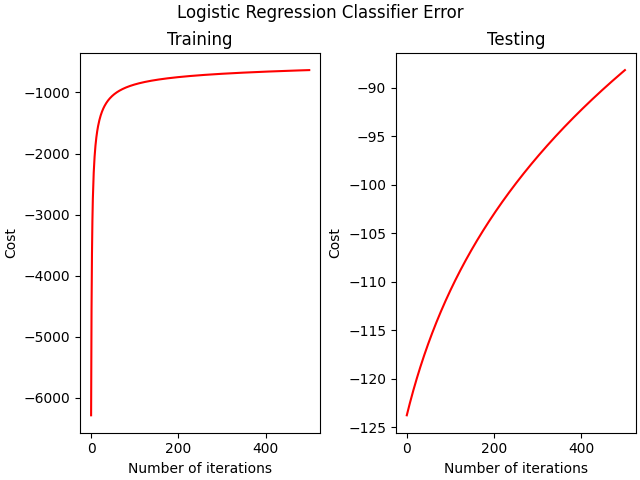
\includegraphics[width=10cm]{logistic_error.png}
	\centering
	\caption{Τα αποτελέσματα της εκπαίδευσης και του ελέγχου στον ταξινομητή μας. Αριστερά: Το κόστος εκπαίδευσης ως συνάρτηση των επαναλήψεων του αλγορίθμου gradient ascent. Δεξία: Το αντίστοιχο κόστος ελέγχου. Υπενθυμίζουμε ότι οι κλίμακες των γραφημάτων δεν είναι ίσες, καθώς ο ήδη εκπαιδευμένος ταξινομητής αρχίζει με πολύ μικρότερο κόστος. }
	\label{logistic_train_test}
\end{figure}


\subsection{Ερώτημα Ε}
Επιλέγουμε το διάστημα των \code{$\lambda$} τιμών μας λογαριθμικά, εφόσον η βέλτιστη τιμή κανονικοποίησης είναι πολύ πιο πιθανό να βρίσκεται αρκετά κοντά στο 0. Η λογαριθμική κλίμακα μας επιτρέπει να ψάξουμε πιο πολλές τιμές του \code{$\lambda$} όσο πιο κοντά φτάνουμε στο κάτω όριο αναζήτησης μας, το $10^{4}$. Η προσέγγιση αυτή χρησιμοποιείται και στην πράξη για κανονικοποίηση $L^{2}$ \cite{jerome}\par

Σημειώνουμε ότι λόγω υπολογιστικών απαιτήσεων, ο αριθμός επαναλήψεων των μοντέλων μας μειώνεται στις 250 επαναλήψεις. Κατά την εκτέλεση του προγράμματος υπάρχει επίσης πιθανότητα να εμφανιστούν ειδοποιήσεις για αριθμητική υπερχείλιση. Αυτό είναι αποτέλεσμα της επιλογής πολύ μεγάλης τιμής του \code{$\lambda$}, κυρίως στο διάστημα [8, 10]. Σε αυτό το σημείο η κανονικοποίηση είναι τόσο ισχυρή που αποτρέπει το μοντέλο μας από το να μάθει, και έτσι αυτό μαντεύει την ίδια κατηγορία για κάθε παράδειγμα ελέγχου.\par

Στην δική μας περίπτωση το μοντέλο, κρατώντας τις υπόλοιπες υπερπαραμέτρους ίσες με το προηγούμενο υποερώτημα, προτιμά την ελάχιστη τιμή κανονικοποίησης \code{$\lambda = 10^{-4}$} με  ακρίβεια ελέγχου ίση με $0.981$. Παρατηρούμε ότι η ακρίβεια ελέγχου με την επιλεγμένη τιμή \code{$\lambda$} είναι μικρότερη από την αντίστοιχη στο υποερώτημα Δ. Αυτό μας υποδεικνύει είτε ότι η βέλτιστη τιμή βρίσκεται έξω (και πιο συγκεκριμένα πριν) από το διάστημα αναζήτησης μας, είτε ότι για την διαφορά ευθύνεται το στατιστικό σφάλμα. \par

Ο κώδικας παραγωγής των παραπάνω γραφημάτων και αποτελεσμάτων βρίσκεται στο αρχείο \code{run\_logistic.py}. Τα πλήρη αποτελέσματα αναζήτησης της υπερπαραμέτρου παρουσιάζονται στην Εικόνα \ref{logistic_lambda_accuracy}.

\begin{figure}
	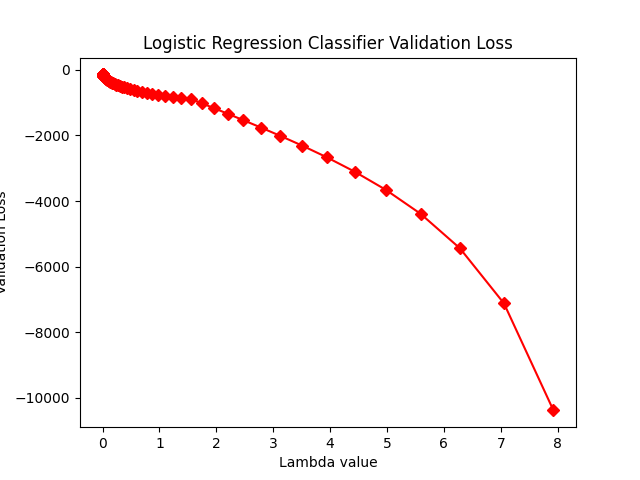
\includegraphics[width=10cm]{logistic_lambda_accuracy.png}
	\centering
	\caption{ Τα αποτελέσματα της αναζήτησης για το βέλτιστο \code{$\lambda$}. Οι ρόμβοι αντιπροσωπεύουν τις τιμές που εξετάσαμε. Παρατηρείστε το πλήθος των τιμών που εξετάστηκαν στην αρχή συγκριτικά με το τέλος του πεδίου αναζήτησής μας.}
	\label{logistic_lambda_accuracy}
\end{figure}


\section{ΜΕΡΟΣ Γ}

\subsection{Ερώτημα ΣΤ}

Το νευρωνικό μας δίκτυο έχει υλοποιηθεί στο αρχείο \code{mlp.py}. Αποτελείται από δύο πίνακες βαρών και δύο πίνακες bias:
\begin{itemize}
	\item  Ο πίνακας \code{h\_w} (hidden weights) έχει μέγεθος $IxH$
	\item  Ο πίνακας \code{o\_w} (output weights) έχει μέγεθος $HxO$
	\item  Ο πίνακας \code{h\_b} (hidden bias) έχει μέγεθος $1xH$
	\item  Ο πίνακας \code{o\_b} (output bias) έχει μέγεθος $1xO$
\end{itemize}
όπου I=\code{input\_size}, H= \code{hidden\_layer\_size}, O= \code{output\_size}. Ο κώδικας για την εκτέλεση του δικτύου βρίσκεται στο αρχείο \code{run\_mlp.py}, το οποίο εκτελεί κώδικα και για τα ερωτήματα Η, Θ.

Θα τρέξουμε το μοντέλο με υπερπαραμέτρους \code{m=2}, \code{$\eta$=0.2} και \code{tolerance=0.001}. Το \code{tolerance} είναι μια υπερ-παράμετρος απαραίτητη για το early stopping, και η οποία καθορίζει πόσο το κόστος πρέπει να έχει μειωθεί για να θεωρείται η τρέχουσα εποχή "βελτίωση". Το αποτέλεσμα είναι η ακρίβεια εκπαίδευσης να είναι ίση με $0.978$, το τελικό κόστος εκπαίδευσης ίσο με $0.0671$, η ακρίβεια ελέγχου ίση με $0.974$ και το μέσο κόστος ελέγχου ίσο με $0.0734$. Τα πλήρη αποτελέσματα της εκπαίδευσης παρουσιάζονται στην Εικόνα \ref{mlp_train_test}.

\begin{figure}
	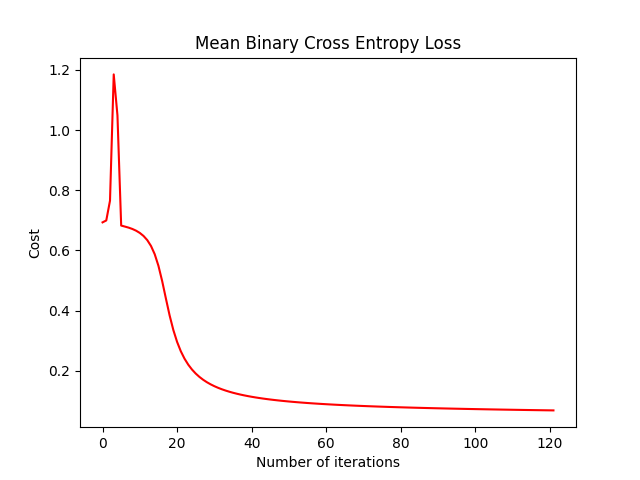
\includegraphics[width=10cm]{mlp_error.png}
	\centering
	\caption{Το κόστος εκπαίδευσης ως συνάρτηση των επαναλήψεων του αλγορίθμου gradient descent.}
	\label{mlp_train_test}
\end{figure}


\subsection{Ερώτημα Ζ}

Ο τύπος της Δυαδικής Διασταυρούμενης Εντροπίας είναι:
\begin{equation}
	\label{eq:1}
	E_{b} = -(t \ln \hat{y} + (1-t) \ln(1-\hat{y}))
\end{equation}
όπου $t$ το διάνυσμα των ετικετών δεδομένων και $\hat{y}$ το της εκτιμώμενης πιθανότητας.

Στην παραπάνω εξίσωση παρατηρούμε ότι η τιμή $t$ είναι πάντοτε γνωστή, αντίθετα με τη $\hat{y}$, επομένως θα παραγωγίσουμε με βάση το $\hat{y}$. Εφόσον $y = f(x) + g(x) \iff y' = f'(x) + g'(x)$ ισχύει ότι:

\begin{equation}
	\label{eq:2}
	\frac{\partial E_b}{\partial \hat{y}} = \frac{\partial}{\partial \hat{y}} (t\ln \hat{y}) + \frac{\partial}{\partial \hat{y}} (1-t) \ln (1-\hat{y})
\end{equation}

Αναλύουμε τις επιμέρους συναρτήσεις του αθροίσματος της παραγώγου:

\begin{equation}
	\label{eq:3}
	\frac{\partial}{\partial \hat{y}} (t \ln\hat{y}) = \frac{\partial }{\hat{y}} (t\ln\hat{y}) + \ln\hat{y} \frac{\partial}{\partial \hat{y}}t = \frac{t}{\hat{y}} + \ln \hat{y} \cdot 0 = \frac{t}{\hat{y}}
\end{equation}

\begin{equation}
	\label{eq:4}
	\frac{\partial}{\partial \hat{y}} ((t-1) \ln(1-\hat{y})) = (1-t)\frac{\partial}{\partial\hat{y}} (\ln(1-\hat{y})) + \ln(1-\hat{y}) \frac{\partial}{\partial \hat{y}}(1-t) = \frac{1-t}{1-\hat{y}} + \ln(1-\hat{y}) \cdot 0 =\frac{1-t}{1-\hat{y}}
\end{equation}


Επομένως, αθροίζοντας τις \ref{eq:3}, \ref{eq:4}, η \ref{eq:2} γίνεται:
\begin{equation}
	\frac{\partial E_b}{\partial \hat{y}} = - (\frac{t}{\hat{y}} - \frac{1-t}{1-\hat{y}}) = (\frac{t}{\hat{y}} + \frac{1-t}{1 - \hat{y}})
\end{equation}

Ο κώδικας επαλήθευσης του αναλυτικού τύπου βρίσκεται στο αρχείο \code{test\_mlp.py}.


\subsection{Ερώτημα Η}

Εκτελούμε grid search για τις παραμέτρους $m, \eta$. Επιλέγουμε το διάστημα των $\eta$ τιμών μας στο χώρο αναζήτησης $[0.5, 10^{-5}]$, εκθετικά κοντά στο $0.5$ εφόσον εμπειρικά αναμένουμε ότι η βέλτιστη τιμή της θα βρίσκεται κοντά στις τιμές $0.5, 0.01, 0.01$.  το οποίο για το συγκεκριμένο δίκτυο είναι το $(\eta=0.5, m=0.5, E=172)$ με κόστος επικύρωσης ίσο με $0.0423$.

Το πρόγραμμα εκτέλεσης του grid search βρίσκεται στο αρχείο \code{run\_mlp.py}. Η αναζήτηση χρειάζεται περίπου 10 λεπτά για να βγάλει το βέλτιστο συνδυασμό υπερπαραμέτρων, το οποίο οφείλεται σχεδόν αποκλειστικά στην εκπαίδευση και επαλήθευση μοντέλων με $M \in {256, 512, 1024}$. Λόγω των περιορισμών στις υπερπαραμέτρους δεν μπορούμε να μειώσουμε σημαντικά τον χρόνο εκτέλεσης.


\subsection{Ερώτημα Θ}

Χρησιμοποιούμε την μέθοδο \code{predict} του μοντέλου μας για να αποκτήσουμε τις προβλεπόμενες ετικέτες του. Η μέθοδος αυτή χρησιμοποιεί μεθόδους της numpy, ισοδύναμες της κατηγοριοποιήσης με βρόγχο. Στο σύνολο ελέγχου το μοντέλο με τις βελτιστοποιημένες παραμέτρους επιτυγχάνει ακρίβεια ελέγχου ίση με $0.979$ και κόστος ελέγχου ίσο με $0.0569$.

\printbibliography

\end{document}